%
% Template Laporan Skripsi/Thesis
%
% @author  Rifa Faruqi
% @version 1.00
%
% Dokumen ini dibuat berdasarkan standar penulisan skripsi Fakultas MIPA, Universitas Syiah Kuala (USK).
% Template ini dimodifikasi dari versi asli yang dibuat oleh Andreas Febrian dan Lia Sadita,
% yang awalnya didasarkan pada standar IEEE dan konfigurasi LaTeX yang digunakan Fahrurrozi Rahman
% untuk laporan skripsi di Universitas Indonesia (UI).
%
% Modifikasi ini disesuaikan dengan panduan terbaru dari Fakultas MIPA, USK.
%
%
% Tipe dokumen adalah report dengan satu kolom. 
%
\documentclass[12pt, a4paper, onecolumn, oneside, final]{report}

% Load konfigurasi LaTeX untuk tipe laporan thesis
\usepackage{_internals/uithesis}


% Daftar pemenggalan suku kata dan istilah dalam LaTeX
%
% Hyphenation untuk Indonesia 
%
% @author  Andreas Febrian
% @version 1.00
% 
% Tambahkan cara pemenggalan kata-kata yang salah dipenggal secara otomatis 
% oleh LaTeX. Jika kata tersebut dapat dipenggal dengan benar, maka tidak 
% perlu ditambahkan dalam berkas ini. Tanda pemenggalan kata menggunakan 
% tanda '-'; contoh:
% menarik
%   --> pemenggalan: me-na-rik
%

\hyphenation{
    % alphabhet A
    a-na-li-sa a-tur 
    a-pli-ka-si 
    % alphabhet B
    ba-ngun-an 
    be-be-ra-pa 
    ber-ge-rak
    ber-ke-lan-jut-an 
    ber-pe-nga-ruh 
    % alphabhet C
    ca-ri copy-writing chat-gpt
    % alphabhet D
    di-sim-pan di-pim-pin de-ngan da-e-rah di-ba-ngun da-pat di-nya-ta-kan 
    di-sim-bol-kan di-pi-lih di-li-hat de-fi-ni-si di-se-su-ai-kan di-ge-ne-ra-si pre-sen-ta-si
    di-ha-rap-kan
    % alphabhet E
    e-ner-gi eks-klu-sif
    % alphabhet F
    fa-si-li-tas
    % alphabhet G
    ga-bung-an ge-rak
    % alphabhet H
    ha-lang-an
    % alphabhet I
    % alphabhet J
    % alphabhet K
    ke-hi-lang-an
    ku-ning 
    kua-li-tas ka-me-ra ke-mung-kin-an ke-se-pa-ham-an
    ke-sempurna-an ke-bu-tu-han
    % alphabhet L
    ling-kung-an
    % alphabhet M
    me-neng-ah
    meng-a-tas-i me-mung-kin-kan me-nge-na-i me-ngi-rim-kan 
    meng-u-bah meng-a-dap-ta-si me-nya-ta-kan mo-di-fi-ka-si
    meng-a-tur meng-ucap-kan ma-nual me-makan meng-or-ga-ni-sa-si-kan mark-down
    mem-ba-ngun
    % alphabhet N
    nya-ta non-eks-klu-sif
    % alphabhet O
    % alphabhet P
	pe-nye-rap-an 
	pe-ngon-trol
    pe-mo-del-an
    pe-ran  pe-ran-an-nya
    pem-ba-ngun-an pre-si-den pe-me-rin-tah prio-ri-tas peng-am-bil-an 
    peng-ga-bung-an pe-nga-was-an pe-ngem-bang-an 
    pe-nga-ruh pa-ra-lel-is-me per-hi-tung-an per-ma-sa-lah-an 
    pen-ca-ri-an peng-struk-tur-an
    per-kembang-an pe-nge-tahu-an 
    po-pu-ler per-ca-kap-an pem-buat-an
    % alphabhet Q
    % alphabhet R
    ran-cang-an res-pons
    % alphabhet S
    si-mu-la-si sa-ngat se-ki-tar
    % alphabhet T
    te-ngah
    ter-da-pat
    % alphabhet U
    % alphabhet V
    % alphabhet W
    % alphabhet X
    % alphabhet Y
    % alphabhet Z
    % special
}

% Load konfigurasi khusus untuk laporan yang sedang dibuat
%-----------------------------------------------------------------------------%
% Informasi Mengenai Dokumen
%-----------------------------------------------------------------------------%
% --------------------
% Informasi Umum
%  -------------------
% Tulis nama penulis 
\var{\penulis}{Rifa Faruqi}
% Tulis kembali nama penulis, kali ini akan diubah menjadi huruf kapital
\Var{\Penulis}{Rifa Faruqi}
\var{\tempatTglLahir}{Banda Aceh/ 29 Maret 2002}
% Tulis NPM penulis
\var{\npm}{21XX}
% Judul laporan. 
% Tuliskan tahun publikasi laporan
\Var{\bulan}{Sep}
\Var{\tahun}{2024}
% Tulis judul 
\var{\judul}{Judul/Topik}
% Tulis kembali judul laporan, kali ini akan diubah menjadi huruf kapital
\Var{\Judul}{Judul/Topik}
% Tulis kembali judul laporan namun dengan bahasa Ingris
\var{\judulInggris}{Judul/Topik}
\var{\JudulInggris}{Judul/Topik}
% Tipe laporan, dapat berisi Skripsi, Tugas Akhir, Thesis, atau Disertasi
\var{\type}{Proposal Penelitian/Tugas Akhir}
\Var{\Type}{Proposal Penelitian/Tugas Akhir}
% 
\var{\jurusan}{Jurusan ?}
% Tulis kembali tipe laporan, kali ini akan diubah menjadi huruf kapital
\Var{\Jurusan}{Jurusan ?}
% Tuliskan gelar yang akan diperoleh dengan menyerahkan laporan ini
\var{\gelar}{Sarjana Ilmu Komputer}
% Tuliskan Fakultas dimana penulis berada
\var{\fakultas}{Matematika dan Ilmu Pengetahuan Alam}
\Var{\Fakultas}{Matematika dan Ilmu Pengetahuan Alam}
% Tuliskan Program Studi yang diambil penulis
\var{\program}{Informatika Jurusan Informatika}
\Var{\Program}{Informatika Jurusan Informatika}
% 
% --------------------------------------------------------
% Informasi untuk halaman pengesahan dan surat pernyataan
% --------------------------------------------------------
% Tuliskan pembimbing 
\var{\pembimbingSatu}{Nama Pembimbing Satu}
\var{\nipPembimbingSatu}{NIP Pemb Satu}
\var{\pembimbingDua}{Nama Pembimbing Dua}
\var{\nipPembimbingDua}{NIP Pemb Dua}
% Infomasi Kaprodi, Dekan dan Koordinator TA
\var{\kaprodi}{Nama Kaprodi}
\var{\kaprodinip}{NIP Kaprodi}
\var{\dekan}{Nama Dekan}
\var{\dekannip}{NIP Dekan}
\var{\koordinatorTA}{Nama Koor TA}
\var{\koordinatorTAnip}{NIP Koor TA}
% Tuliskan tanggal pengesahan
\var{\tanggalPengesahan}{Hari, XX Bulan YYYY} 
% Tanggal pernyataan bebas plagiasi
\var{\tanggalPernyataanBebasPlagiasi}{Banda Aceh, XX Bulan YYYY}
% Tuliskan tanggal keputusan sidang dikeluarkan dan penulis dinyatakan 
% lulus/tidak lulus
\var{\tanggalLulus}{XX Juli 2019}
% 
\var{\tanggalKataPengantar}{Banda Aceh, XX Bulan YYYY}
% 
% Alias untuk memudahkan alur penulisan paa saat menulis laporan
\var{\saya}{Penulis}

%-----------------------------------------------------------------------------%
% Judul Setiap Bab
%-----------------------------------------------------------------------------%
% 
% Berikut ada judul-judul setiap bab. 
% Silahkan diubah sesuai dengan kebutuhan. 
% 
\Var{\kataPengantar}{Kata Pengantar}
\Var{\babSatu}{Pendahuluan}
\Var{\babDua}{Tinjauan Kepustakaan}
\Var{\babTiga}{Metodologi Penelitian}
\Var{\babEmpat}{Hasil dan Pembahasan}
\Var{\babLima}{Kesimpulan dan Saran}

\Var{\babEnam}{Bab Enam}
\Var{\kesimpulan}{Kesimpulan dan Saran}

% Daftar istilah yang mungkin perlu ditandai 
%
% @author  Andreas Febrian
% @version 1.00
% 
% Mendaftar seluruh istilah yang mungkin akan perlu dijadikan 
% italic atau bold pada setiap kemunculannya dalam dokumen. 
% 

\var{\license}{\f{Creative Common License 1.0 Generic}}
\var{\bslash}{$\setminus$}

% Awal bagian penulisan laporan
\begin{document}
%
%
% Gunakan penomeran romawi
\pagenumbering{roman}
\fancyhf{} % Bersihkan header dan footer terlebih dahulu
\fancyfoot[C]{\thepage} % Nomor halaman di tengah bawah (bisa ganti posisi jika diperlukan)


%
% load halaman judul dalam
\addChapter{Halaman Judul}
%
% Halaman Judul Laporan 
%
% @author  unknown
% @version 1.01
% @edit by Andreas Febrian
%

\begin{titlepage}

    \begin{center}
        % judul thesis harus dalam 14pt Times New Roman
        \vspace*{4em}
        {\fontsize{20}{20}
            \textbf{\Judul} \\[3em]
        }
        % Mengatur ukuran font menjadi 16pt dan menambahkan spasi vertikal
        {\fontsize{16}{20}
            \textbf{\Type} \\[3em] 
        }
        % keterangan prasyarat
        {\fontsize{12}{20}
            {Diajukan untuk melengkapi tugas-tugas dan memenuhi syarat-syarat guna memperoleh gelar 
            \gelar} \\[3em]
        }
        % Oleh
        {\fontsize{14}{20}
            {Oleh:} \\[3em]
        }
        % penulis dan npm
        {\fontsize{14}{20}
            \underline{\bo{\Penulis}} \\
            \underline{\bo{\npm}} \\[3em]
        }
        
        \begin{figure}
            \begin{center}
                
\includegraphics[width=4cm]{_internals/usk_logo.png}
            \end{center}
        \end{figure}    
        \vspace*{3em}
        

        % informasi mengenai fakultas dan program studi
        \bo{
            PROGRAM STUDI \Program\ FAKULTAS \Fakultas\\ UNIVERSITAS SYIAH KUALA, BANDA ACEH \\
            \bulan, \tahun
        }
    \end{center}
\end{titlepage}

% setelah bagian ini, halaman dihitung sebagai halaman ke 2
\setcounter{page}{2}
%
% Untuk seminar proposal, uncomment bagian ini
\addChapter{Halaman Pengesahan}
%------------------------------------------------------------
%Approval Page
%------------------------------------------------------------
\chapter*{PENGESAHAN}


\begin{center}
    \begin{doublespace}
        \vspace{0.5cm}
        \fontsize{12pt}{10pt}\selectfont\MakeUppercase{\large{\bfseries\judul}}\par\nobreak

        \vspace{1cm}
        \fontsize{12pt}{10pt}\selectfont\MakeUppercase{\large{\bfseries\judulInggris}}\par\nobreak

        \vspace{0.9cm}
        Oleh:
        %\vspace{-0.5cm}
        \begin{singlespace}
            \begin{compactitem}
                \addtolength{\itemindent}{3cm}
                \setlength{\parsep}{0pt}
                \item[]{\makebox[2cm]{Nama\hfill} : \penulis}
                \item[]{\makebox[2cm]{NPM\hfill} : \npm}
                \item[]{\makebox[2cm]{Jurusan\hfill} : \jurusan}
            \end{compactitem}
        \end{singlespace}
        %\vspace{2.0cm} edited 16/04/2022
        \vspace{0.9cm}
        
        %Telah disetujui dan disahkan\\
        %\vspace{1.0cm}

        Menyetujui:\\
        \onehalfspacing
            \begin{tabular}{lll}
                Pembimbing I & \hspace{2.5cm} & Pembimbing II \\
                \vspace{0.3cm} & \vspace{0.3cm} & \vspace{0.3cm}\\
                \underline{\pembimbingSatu}& &
                \underline{\pembimbingDua} \\
                NIP. \nipPembimbingSatu & &  NIP. \nipPembimbingDua
            \end{tabular}	
        %\vspace{2.0cm} edited 16/04/2022
        \vspace{0.5cm}
        
        % Mengetahui dekan dan kajur informatika
        % Tanpa mengetahui dekan
        Mengetahui:\\
        Koordinator Prodi S1 Informatika FMIPA\\
        Universitas Syiah Kuala,\\
        \vspace{4em}
        \underline{\kaprodi}\\
        NIP. \kaprodinip
    \end{doublespace}

\end{center}

\thispagestyle{empty}   % Mematikan penomoran halaman
% 
% -- Halaman Pengesahan untuk sidang
\addChapter{Halaman Pengesahan}
%------------------------------------------------------------
%Approval Page
%------------------------------------------------------------
\chapter*{PENGESAHAN}


\begin{center}
    \begin{doublespace}
        \vspace{0.5cm}
        \fontsize{12pt}{10pt}\selectfont\MakeUppercase{\large{\bfseries\judul}}\par\nobreak

        \vspace{1cm}
        \fontsize{12pt}{10pt}\selectfont\MakeUppercase{\large{\bfseries\judulInggris}}\par\nobreak

        \vspace{0.9cm}
        Oleh:
        %\vspace{-0.5cm}
        \begin{singlespace}
            \begin{compactitem}
                \addtolength{\itemindent}{3cm}
                \setlength{\parsep}{0pt}
                \item[]{\makebox[2cm]{Nama\hfill} : \penulis}
                \item[]{\makebox[2cm]{NPM\hfill} : \npm}
                \item[]{\makebox[2cm]{Jurusan\hfill} : \jurusan}
            \end{compactitem}
        \end{singlespace}
        %\vspace{2.0cm} edited 16/04/2022
        \vspace{0.9cm}
        
        %Telah disetujui dan disahkan\\
        %\vspace{1.0cm}

        Menyetujui:\\
        \onehalfspacing
            \begin{tabular}{lll}
                Pembimbing I & \hspace{2.5cm} & Pembimbing II \\
                \vspace{0.3cm} & \vspace{0.3cm} & \vspace{0.3cm}\\
                \underline{\pembimbingSatu}& &
                \underline{\pembimbingDua} \\
                NIP. \nipPembimbingSatu & &  NIP. \nipPembimbingDua
            \end{tabular}	
        %\vspace{2.0cm} edited 16/04/2022
        \vspace{1.0cm}
        
        % Mengetahui dekan dan kajur informatika
        % Tanpa mengetahui dekan
        Mengetahui:\\
            \begin{tabular}{lll}
                Dekan FMIPA & &
                Koordinator Prodi S1 Informatika FMIPA \\ 
                \vspace{-0.27cm} & \vspace{-0.27cm} & \vspace{-0.27cm}\\
                Universitas Syiah Kuala, & & Universitas Syiah Kuala,\\
                \vspace{0.3cm} & \vspace{0.3cm} & \vspace{0.3cm}\\
                \underline{\dekan} & & \underline{\kaprodi}\\
                    NIP. \dekannip & & NIP. \kaprodinip
            \end{tabular}
    \end{doublespace}

    \vspace{0.9cm}
    Lulus Sidang Sarjana pada hari \tanggalPengesahan
\end{center}

\thispagestyle{empty}   % Mematikan penomoran halaman

% --- Surat pernyataan bebas plagiasi 
\addChapter{Pernyataan Bebas Plagiasi}
\chapter*{PERNYATAAN BEBAS PLAGIASI}


\noindent
Saya yang bertanda tangan di bawah ini,

\vspace{-0.1cm}

\begin{table}[H]
\begin{tabular}{ll}
    \textbf{Nama lengkap}          &: \penulis \\
    \textbf{Tempat/tanggal lahir}   &: \tempatTglLahir \\
    \textbf{NPM}                   &: \npm    \\
    \textbf{Program Studi}          &: \jurusan \\
    \textbf{Fakultas}               &: \fakultas \\
    \textbf{Judul Tugas Akhir}      &: 
    \parbox[t]{0.67\textwidth}{
        \Judul
    }
\end{tabular}
\end{table}

\vspace{0.2cm}
\noindent
Menyatakan dengan sesungguhnya bahwa Laporan Tugas Akhir saya dengan judul di atas adalah \textbf{hasil karya saya sendiri} bersama dosen pembimbing dan \textbf{bebas plagiasi}.

\vspace{1cm}
\noindent
Jika ternyata di kemudian hari terbukti bahwa Laporan Tugas Akhir merupakan hasil plagiasi, saya bersedia menerima sanksi yang berlaku di Universitas Syiah Kuala.

\vspace{1cm}


\begin{tabular}{p{7.5cm}l}
	&\tanggalPernyataanBebasPlagiasi\\
	&\\
	&\\
	&\multirow{1.5}{7.5cm}{\underline{\penulis}} \\ 
	&NPM. \npm \\
\end{tabular}
\thispagestyle{empty}   % Mematikan penomoran halaman

% --- Surat pernyataan
\addChapter{Surat Pernyataan}
\chapter*{SURAT PERNYATAAN}

\begin{singlespace}

\noindent
Yang bertanda tangan di bawah ini,
\vspace{-0.1cm}

\begin{table}[H]
\centering
\begin{tabularx}{\textwidth}{llX} % X untuk kolom yang dapat menyesuaikan
1. &   Nama  		&: \penulis \\
	&   NPM       	&: \npm   \\
	&   Jurusan/Prodi &: \jurusan \\
	&   Status      	&: Mahasiswa \\  
2.	& Nama  		&: \pembimbingSatu \\
	&   NIP       	&: \nipPembimbingSatu   \\
	&   Jurusan/Prodi &: Informatika \\
	&   Status      	&: Pembimbing I \\  
3.	& Nama  		&: \pembimbingDua \\
	&   NIP       	&: \nipPembimbingDua   \\
	&   Jurusan/Prodi &: Informatika \\
	&   Status      	&: Pembimbing II   
\end{tabularx}
\end{table}

\vspace{-0.4cm}
\noindent
Dengan ini menyatakan hasil penelitian Tugas Akhir yang berjudul \textbf{\Judul} tidak dipublikasikan secara \textit{full-text} di sistem ETD (\textit{Electronic Theses and Dissertations}) Universitas Syiah Kuala hingga batas waktu 5 tahun dari tanggal kelulusan.

\vspace{0.4cm}
\noindent
Demikian surat pernyataan ini dibuat dengan sebenarnya untuk dapat dipergunakan seperlunya.

\vspace{0.4cm}
{\renewcommand{\arraystretch}{0.8}
\centering
\begin{tabularx}{\textwidth}{llX} % X untuk kolom yang dapat menyesuaikan
	&\tanggalSuratPernyataan		& \\
	&Yang membuat pernyataan,			& \\
	&&\\
	Pembimbing I,							&Pembimbing II,							&Mahasiswa,\\
	&&\\
	&&\\
	&&\\
	\underline{\pembimbingSatu}	&\underline{\pembimbingDua} &\underline{\penulis}\\
	NIP. \nipPembimbingSatu				&NIP. \nipPembimbingDua				&NPM. \npm \\
	&&\\
	&Mengetahui:\\			&
\end{tabularx}
}
{\renewcommand{\arraystretch}{0.8}
\begin{tabularx}{\textwidth}{llX} % X untuk kolom yang dapat menyesuaikan
	Koordinator Program Studi Informatika	&\qquad\qquad  &Koordinator TA,\\
	Universitas Syiah Kuala,&\quad\quad  &\\
	&&\\
	&&\\
	&&\\
	\underline{\kaprodi}	&\quad\quad  &\underline{\koordinatorTA}\\
	NIP. \kaprodinip						&\quad\quad  &NIP. \koordinatorTAnip				
\end{tabularx}
}
\end{singlespace}
\thispagestyle{empty}   % Mematikan penomoran halaman

% --- Bagian Abstrak
\addChapter{Abstrak/Abstract}
%
% Halaman Abstrak
%
% @author  Andreas Febrian
% @version 1.00
%

\chapter*{Abstrak}



\begin{singlespace} % Atur 1 spasi untuk bagian abstract sesuai pedoman
{

	Tesis ini membahas kemampuan mahasiswa Fakultas Psikologi UI dalam mencari dan
	menggunakan informasi secara efektif dalam konteks \textit{active learning} dan \textit{self regulated
	learning} selama mereka mengikuti Program Pendidikan Dasar Pendidikan Tinggi.
	Penelitian ini adalah penelitian kualitatif dengan desain deskriptif. Hasil penelitian
	menyarankan bahwa perpustakaan perlu dilibatkan dalam pengembangan kurikulum;
	materi pendidikan pemakai perpustakaan harus dikembangkan sesuai dengan komponen-
	komponen yang ada dalam \textit{information literacy}; perpustakaan juga harus menyediakan
	sarana dan fasilitas yang mendukung peningkatan \textit{literacy} mahasiswa. \\ \\
    Kata kunci:
	Informasi, \textit{information literacy}, \textit{information skills}
}
\end{singlespace}

%
% Halaman Abstract
%
% @author  Andreas Febrian
% @version 1.00
%

\begin{singlespace} % Atur 1 spasi untuk bagian abstract sesuai pedoman
\chapter*{Abstract}


{
	The focus of this study is the freshman student of Faculty of Psychology at University of
	Indonesia experience of acquiring, evaluating and using information, when they enroll in
	“Program Dasar Pendidikan Tinggi (PDPT)”. The purpose of this study is to understand
	how freshman students acquire, evaluate and use information. Knowing this will allow
	library to identify changes should be made to improve user education program at
	University of Indonesia. This research is qualitative descriptive interpretive. The data
	were collected by means of deep interview. The researcher suggests that library should
	improve the user education program and provide facilities which can help students to be
	information literate. \\ \\
Key words:
	Information literacy, information skills, information
}
\end{singlespace}
\newpage

% --- Bagian Kata Pengantar
\addChapter{Kata Pengantar}
%-----------------------------------------------------------------------------%
\chapter*{Kata Pengantar}


%-----------------------------------------------------------------------------%
Template ini disediakan untuk orang-orang yang berencana menggunakan 
\latex~untuk membuat dokumen tugas akhirnya. 
Mengapa \latex? 
Ada banyak hal mengapa menggunakan \latex, diantaranya:

\begin{enumerate}
	\item \latex~membuat kita jadi lebih fokus terhadap isi dokumen, bukan 
		tampilan atau halaman. 
	\item \latex~memudahkan dalam penulisan persamaan matematis. 
	\item Adanya automatis dalam penomoran caption, bab, subbab, subsubbab, 
		referensi, dan rumus. 
	\item Adanya automatisasi dalam pembuatan daftar isi, daftar gambar, dan
		daftar tabel. 
	\item Adanya kemudahan dalam memberikan referensi dalam tulisan dengan 
		menggunakan label. Cara ini dapat meminimalkan kesalahan pemberian 
		referensi. 
\end{enumerate}

Template ini bebas digunakan dan 
didistribusikan sesuai dengan aturan \license, yang secara sederhana berisi: 

\begin{figure}
	\centering
	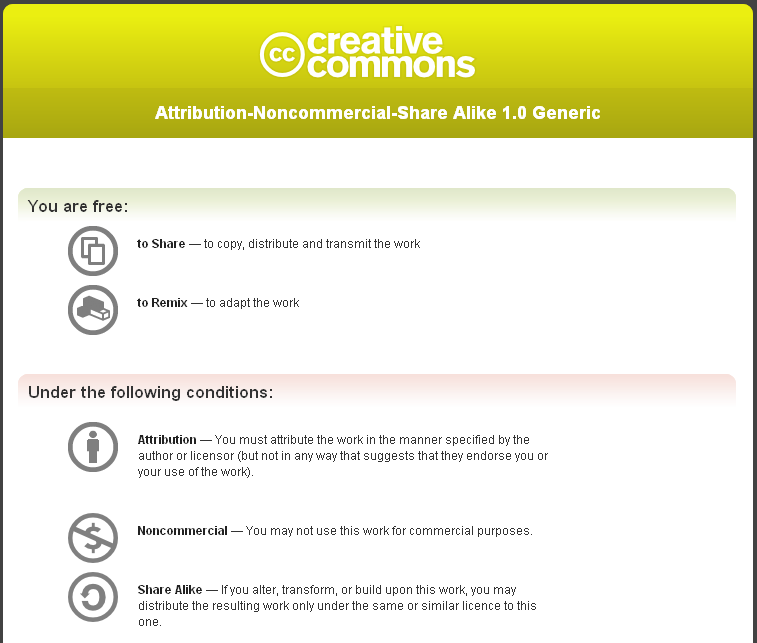
\includegraphics[width=0.74\textwidth]
		{assets/pics/creative_common.png}
	\caption{\license}
	\label{fig:lisensi}
\end{figure}

\pic~\ref{fig:lisensi} diambil dari 
\url{http://creativecommons.org/licenses/by-nc-sa/1.0/deed.en_CA}. 
Jika ingin mengentahui lebih lengkap mengenai \license, silahkan buka 
\url{http://creativecommons.org/licenses/by-nc-sa/1.0/legalcode}. 
Seluruh dokumen yang dibuat dengan menggunakan template ini sepenuhnya 
menjadi hak milik pembuat dokumen dan bebas didistribusikan sesuai dengan 
keperluan masing-masing. 
Lisensi hanya berlaku jika ada orang yang membuat template baru dengan 
menggunakan template ini sebagai dasarnya. 

Dokumen ini dibuat dengan \latex~juga. Untuk meyakinkan Anda, coba lihat 
properti dari dokumen ini dan Anda akan menemukan bagian seperti 
\pic~\ref{fig:pdflatex}. 
Dokumen ini dimaksudkan untuk memberikan gambaran kepada Anda seperti apa 
mudahnya menggunakan \latex~dan juga memperlihatkan betapa bagus dokumen 
yang dihasilkan. 
Seluruh url yang Anda temukan dapat Anda klik. 
Seluruh referensi yang ada juga dapat diklik. 
Untuk mengerti template yang disediakan, Anda tetap harus membuka kode 
\latex~dan bermain-main dengannya. 
Penjelasan dalam PDF ini masih bersifat gambaran dan tidak begitu 
mendetail, dapat dianggap sebagai pengantar singkat. 
Jika Anda merasa kesulitan dengan template ini, mungkin ada baiknya 
Anda belajar sedikit dasar-dasar \latex. 

\begin{figure}
	\centering
	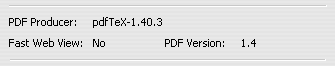
\includegraphics[width=0.54\textwidth]
		{assets/pics/mark.png}
	\caption{Dokumen Dibuat dengan PDFLatex}
	\label{fig:pdflatex}
\end{figure}

Semoga template ini dapat membantu orang-orang yang ingin mencoba menggunakan 
\latex. Semoga template ini juga tidak berhenti disini dengan ada kontribusi 
dari para penggunanya. 
Kami juga ingin berterima kasih kepada Andreas Febrian, Lia Sadita, Fahrurrozi 
Rahman, Andre Tampubolon, dan Erik Dominikus atas kontribusinya dalam template 
ini. 

\vspace*{0.1cm}
\begin{tabular}{p{7.5cm}l}
	&\tanggalKataPengantar\\
	&\\
	&\\
	&\multirow{1.5}{7.5cm}{\underline{\penulis}} \\ 
	&NPM. \npm \\
\end{tabular}
%
%
%
% Daftar isi, gambar, dan tabel
%
% Atur jarak antar chapter sama seperti jarak antar section
\disableboldchapterintoc
\phantomsection
\begin{singlespace}
\tableofcontents
\clearpage

\phantomsection
\listoftables
\clearpage

\phantomsection
\listoffigures
\clearpage

\phantomsection
\listofappendices
\addcontentsline{toc}{chapter}{Daftar Lampiran}
\clearpage

\enableboldchapterintoc

\end{singlespace}

%
% Gunakan penomeran Arab (1, 2, 3, ...) setelah bagian ini.
%
\pagenumbering{arabic} % Mengatur penomoran halaman ke format Arab
\fancyhf{} % Bersihkan header dan footer
\fancyfoot[R]{\thepage} % Nomor halaman di kanan bawah
%
%
%
%-----------------------------------------------------------------------------%
\chapter{\babSatu}
\thispagestyle{fancy}
%-----------------------------------------------------------------------------%
\todo{tambahkan kata-kata pengantar bab 1 disini}


%-----------------------------------------------------------------------------%
\section{Latar Belakang}
%-----------------------------------------------------------------------------%
\todo{tuliskan latar belakang penelitian disini}


%-----------------------------------------------------------------------------%
\section{Permasalahan}
%-----------------------------------------------------------------------------%
Pada bagian ini akan dijelaskan mengenai definisi permasalahan 
yang \saya~hadapi dan ingin diselesaikan serta asumsi dan batasan 
yang digunakan dalam menyelesaikannya.


%-----------------------------------------------------------------------------%
\subsection{Definisi Permasalahan}
%-----------------------------------------------------------------------------%
\todo{Tuliskan permasalahan yang ingin diselesaikan. Bisa juga
	berbentuk pertanyaan}


%-----------------------------------------------------------------------------%
\subsection{Batasan Permasalahan}
%-----------------------------------------------------------------------------%
\todo{Umumnya ada asumsi atau batasan yang digunakan untuk 
	menjawab pertanyaan-pertanyaan penelitian diatas.}


%-----------------------------------------------------------------------------%
\section{Tujuan}
%-----------------------------------------------------------------------------%
\todo{Tuliskan tujuan penelitian.}


%-----------------------------------------------------------------------------%
\section{Posisi Penelitian}
%-----------------------------------------------------------------------------%
\todo{Posisi penelitian Anda jika dilihat secara bersamaan dengan 
	peneliti-peneliti lainnya. Akan lebih baik lagi jika ikut menyertakan 
	diagram yang menjelaskan hubungan dan keterkaitan antar 
	penelitian-penelitian sebelumnya}


%-----------------------------------------------------------------------------%
\section{Metodologi Penelitian}
%-----------------------------------------------------------------------------%
\todo{Tuliskan metodologi penelitian yang digunakan.}


%-----------------------------------------------------------------------------%
\section{Sistematika Penulisan}
%-----------------------------------------------------------------------------%
Sistematika penulisan laporan adalah sebagai berikut:
\begin{itemize}
	\item Bab 1 \babSatu \\
	\item Bab 2 \babDua \\
	\item Bab 3 \babTiga \\
	\item Bab 4 \babEmpat \\
	\item Bab 5 \babLima \\
	\item Bab 6 \babEnam \\
	\item Bab 7 \kesimpulan \\
\end{itemize}

\todo{Tambahkan penjelasan singkat mengenai isi masing-masing bab.}


%-----------------------------------------------------------------------------%
\chapter{\babDua}
\thispagestyle{fancy}
%-----------------------------------------------------------------------------%
\todo{tambahkan kata-kata pengantar bab 2 disini}

%-----------------------------------------------------------------------------%
\section{\latex~Secara Singkat}
%-----------------------------------------------------------------------------%
Definisi dari LaTeX \citep{lankton2008introduction} adalah: \\ 
\begin{tabular}{| p{13cm} |}
	\hline 
	\\
	LaTeX is a family of programs designed to produce publication-quality 
	typeset documents. It is particularly strong when working with 
	mathematical symbols. \\	
	The history of LaTeX begins with a program called TEX. In 1978, a 
	computer scientist by the name of Donald Knuth grew frustrated with the 
	mistakes that his publishers made in typesetting his work. He decided 
	to create a typesetting program that everyone could easily use to 
	typeset documents, particularly those that include formulae, and made 
	it freely available. The result is TEX. \\	
	Knuth's product is an immensely powerful program, but one that does 
	focus very much on small details. A mathematician and computer 
	scientist by the name of Leslie Lamport wrote a variant of TEX called 
	LaTeX that focuses on document structure rather than such details. \\
	\\
	\hline
\end{tabular}

\vspace*{0.8cm}

Contoh sitasi lainnya menggunakan \verb|\citep| adalah saat kita mau mensitasi pekerjaan tentang \textit{machine learning} \citep{chin2000learning} dan \textit{dynamic programming} \citep{barto1995learning}. \\

Dokumen \latex~sangat mudah, seperti halnya membuat dokumen teks biasa. Ada 
beberapa perintah yang diawali dengan tanda '\bslash'. 
Seperti perintah \bslash\bslash~yang digunakan untuk memberi baris baru. 
Perintah tersebut juga sama dengan perintah \bslash newline. 
Pada bagian ini akan sedikit dijelaskan cara manipulasi teks dan 
perintah-perintah \latex~yang mungkin akan sering digunakan. 
Jika ingin belajar hal-hal dasar mengenai \latex, silahkan kunjungi: 

\begin{itemize}
	\item \url{http://frodo.elon.edu/tutorial/tutorial/}, atau
	\item \url{http://www.maths.tcd.ie/~dwilkins/LaTeXPrimer/}
\end{itemize}


%-----------------------------------------------------------------------------%
\section{\latex~Kompiler dan IDE}
%-----------------------------------------------------------------------------%
Agar dapat menggunakan \latex~(pada konteks hanya sebagai pengguna), Anda 
tidak perlu banyak tahu mengenai hal-hal didalamnya. 
Seperti halnya pembuatan dokumen secara visual (contohnya Open Office (OO) 
Writer), Anda dapat menggunakan \latex~dengan cara yang sama. 
Orang-orang yang menggunakan \latex~relatif lebih teliti dan terstruktur 
mengenai cara penulisan yang dia gunakan, \latex~memaksa Anda untuk seperti 
itu.  

Kembali pada bahasan utama, untuk mencoba \latex~Anda cukup mendownload 
kompiler dan IDE. Saya menyarankan menggunakan Texlive dan Texmaker. 
Texlive dapat didownload dari \url{http://www.tug.org/texlive/}. 
Sedangkan Texmaker dapat didownload dari 
\url{http://www.xm1math.net/texmaker/}. 
Untuk pertama kali, coba buka berkas thesis.tex dalam template yang Anda miliki 
pada Texmaker. 
Dokumen ini adalah dokumen utama. 
Tekan F6 (PDFLaTeX) dan Texmaker akan mengkompilasi berkas tersebut menjadi 
berkas PDF. 
Jika tidak bisa, pastikan Anda sudah menginstall Texlive. 
Buka berkas tersebut dengan menekan F7. 
Hasilnya adalah sebuah dokumen yang sama seperti dokumen yang Anda baca saat 
ini. 


%-----------------------------------------------------------------------------%
\section{Bold, Italic, dan Underline}
%-----------------------------------------------------------------------------%
Hal pertama yang mungkin ditanyakan adalah bagaimana membuat huruf tercetak 
tebal, miring, atau memiliki garis bawah. 
Pada Texmaker, Anda bisa melakukan hal ini seperti halnya saat mengubah dokumen 
dengan OO Writer. 
Namun jika tetap masih tertarik dengan cara lain, ini dia: 

\begin{itemize}
	\item \bo{Bold} \\
		Gunakan perintah \bslash textbf$\lbrace\rbrace$ atau 
		\bslash bo$\lbrace\rbrace$. 
	\item \f{Italic} \\
		Gunakan perintah \bslash textit$\lbrace\rbrace$ atau 
		\bslash f$\lbrace\rbrace$. 
	\item \underline{Underline} \\
		Gunakan perintah \bslash underline$\lbrace\rbrace$.
	\item $\overline{Overline}$ \\
		Gunakan perintah \bslash overline. 
	\item $^{superscript}$ \\
		Gunakan perintah \bslash $\lbrace\rbrace$. 
	\item $_{subscript}$ \\
		Gunakan perintah \bslash \_$\lbrace\rbrace$. 
\end{itemize}

Perintah \bslash f dan \bslash bo hanya dapat digunakan jika package 
uithesis digunakan. 


%-----------------------------------------------------------------------------%
\section{Memasukan Gambar}
%-----------------------------------------------------------------------------%
Setiap gambar dapat diberikan caption dan diberikan label. Label dapat 
digunakan untuk menunjuk gambar tertentu. 
Jika posisi gambar berubah, maka nomor gambar juga akan diubah secara 
otomatis. 
Begitu juga dengan seluruh referensi yang menunjuk pada gambar tersebut. 
Contoh sederhana adalah \pic~\ref{fig:testGambar}. 
Silahkan lihat code \latex~dengan nama bab2.tex untuk melihat kode lengkapnya. 
Harap diingat bahwa caption untuk gambar selalu terletak dibawah gambar. 

\begin{figure}
	\centering
	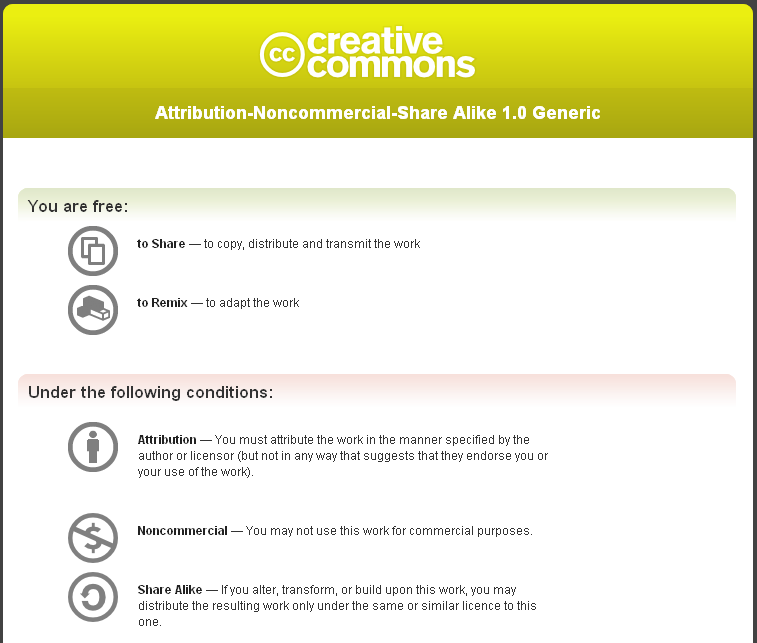
\includegraphics[width=0.50\textwidth]
		{assets/pics/creative_common.png}
	\caption{\license.}
	\label{fig:testGambar}
\end{figure}


%-----------------------------------------------------------------------------%
\section{Membuat Tabel}
%-----------------------------------------------------------------------------%
Seperti pada gambar, tabel juga dapat diberi label dan caption. 
Caption pada tabel terletak pada bagian atas tabel. 
Contoh tabel sederhana dapat dilihat pada \tab~\ref{tab:tab1}.

\begin{table}
	\centering
	\caption{Contoh Tabel}
	\label{tab:tab1}
	\begin{tabular}{| l | c r |}
		\hline
		& kol 1 & kol 2 \\ 
		\hline
		baris 1 & 1 & 2 \\
		baris 2 & 3 & 4 \\
		baris 3 & 5 & 6 \\
		jumlah  & 9 & 12 \\
		\hline
	\end{tabular}
\end{table}

Ada jenis tabel lain yang dapat dibuat dengan \latex~berikut 
beberapa diantaranya. 
Contoh-contoh ini bersumber dari 
\url{http://en.wikibooks.org/wiki/LaTeX/Tables}

\begin{table}
	\centering
	\caption{An Example of Rows Spanning Multiple Columns}
	\label{row.spanning}
	\begin{tabular}{|l|l|*{6}{c|}}
  		\hline % create horizontal line
  		No & Name & \multicolumn{3}{|c|}{Week 1} & \multicolumn{3}{|c|}{Week 2} \\
  		\cline{3-8} % create line from 3rd column till 8th column
  		& & A & B & C & A & B & C\\
  		\hline
  		1 & Lala & 1 & 2 & 3 & 4 & 5 & 6\\
  		2 & Lili & 1 & 2 & 3 & 4 & 5 & 6\\
  		3 & Lulu & 1 & 2 & 3 & 4 & 5 & 6\\
  		\hline
	\end{tabular}
\end{table}

\begin{table}
	\centering
	\caption{An Example of Columns Spanning Multiple Rows}
	\label{column.spanning}
	\begin{tabular}{|l|c|l|}
		\hline
		Percobaan & Iterasi & Waktu \\
		\hline
		Pertama & 1 & 0.1 sec \\ \hline
		\multirow{2}{*}{Kedua} & 1 & 0.1 sec \\
 		& 3 & 0.15 sec \\ 
 		\hline
		\multirow{3}{*}{Ketiga} & 1 & 0.09 sec \\
 		& 2 & 0.16 sec \\
 		& 3 & 0.21 sec \\ 
 		\hline
	\end{tabular}
\end{table}

\begin{table}
	\centering
	\caption{An Example of Spanning in Both Directions Simultaneously}
	\label{mix.spanning}
	\begin{tabular}{cc|c|c|c|c|}
		\cline{3-6}
		& & \multicolumn{4}{|c|}{Title} \\ \cline{3-6}
		& & A & B & C & D \\ \hline
		\multicolumn{1}{|c|}{\multirow{2}{*}{Type}} &
		\multicolumn{1}{|c|}{X} & 1 & 2 & 3 & 4\\ \cline{2-6}
		\multicolumn{1}{|c|}{}                        &
		\multicolumn{1}{|c|}{Y} & 0.5 & 1.0 & 1.5 & 2.0\\ \cline{1-6}
		\multicolumn{1}{|c|}{\multirow{2}{*}{Resource}} &
		\multicolumn{1}{|c|}{I} & 10 & 20 & 30 & 40\\ \cline{2-6}
		\multicolumn{1}{|c|}{}                        &
		\multicolumn{1}{|c|}{J} & 5 & 10 & 15 & 20\\ \cline{1-6}
	\end{tabular}
\end{table}


%-----------------------------------------------------------------------------%
\chapter{\babTiga}
\thispagestyle{fancy}
%-----------------------------------------------------------------------------%
\todo{tambahkan kata-kata pengantar bab 1 disini}


%-----------------------------------------------------------------------------%
\section{Satu Persamaan}
%-----------------------------------------------------------------------------%

\noindent \begin{align}\label{eq:garis}
	\cfrac{y - y_{1}}{y_{2} - y_{1}} = 
	\cfrac{x - x_{1}}{x_{2} - x_{1}}
\end{align}

\equ~\ref{eq:garis} diatas adalah persamaan garis. 
\equ~\ref{eq:garis} dan \ref{eq:bola} sama-sama dibuat dengan perintah \bslash
align. 
Perintah ini juga dapat digunakan untuk menulis lebih dari satu persamaan. 

\noindent \begin{align}\label{eq:bola}
	\underbrace{|\overline{ab}|}_{\text{pada bola $|\overline{ab}| = r$}} 
		= \sqrt[2]{(x_{b} - x_{a})^{2} + (y_{b} - y_{a})^{2} + 
				\vert\vert(z_{b} - z_{a})^{2}}
\end{align}

%-----------------------------------------------------------------------------%
\section{Lebih dari Satu Persamaan}
\label{sec:multiEqu}
%-----------------------------------------------------------------------------%
\noindent \begin{align}\label{eq:matriks}	
	|\overline{a} * \overline{b}| &= |\overline{a}| |\overline{b}| \sin\theta 
		\\[0.2cm]
	\overline{a} * \overline{b} &=  
		\begin{array}{| c c c |}
			\hat{i} & x_{1} & x_{2} \\
			\hat{j} & y_{1} & y_{2} \\
			\hat{k} & z_{1} & z_{2} \\
		\end{array} \nonumber \\[0.2cm]
	&= \hat{i} \,
		\begin{array}{ | c c | }
			y_{1} & y_{2} \\
			z_{1} & z_{2} \\
		\end{array} 
	   + \hat{j} \,
		\begin{array}{ | c c | }
			z_{1} & z_{2} \\
			x_{1} & x_{2} \\
		\end{array} 
	   + \hat{k} \,	
		\begin{array}{ | c c | }
			x_{1} & x_{2} \\
			y_{1} & y_{2} \\
		\end{array}
		\nonumber
\end{align}

Pada \equ~\ref{eq:matriks} dapat dilihat beberapa baris menjadi satu bagian 
dari \equ~\ref{eq:matriks}. 
Sedangkan dibawah ini dapat dilihat bahwa dengan cara yang sama, \equ~
\ref{eq:gabungan1}, \ref{eq:gabungan2}, dan \ref{eq:gabungan3} memiliki nomor 
persamaannya masing-masing. 

\noindent \begin{align}\label{eq:gabungan1}	
	\int_{a}^{b} f(x)\, dx + \int_{b}^{c} f(x) \, dx = \int_{a}^{c} f(x) \, dx
		\\\label{eq:gabungan2}
	\lim_{x \to \infty} \frac{f(x)}{g(x)} = 0 \hspace{1cm} 
		\text{jika pangkat $f(x)$ $<$ pangkat $g(x)$} \\\label{eq:gabungan3}
	a^{m^{a \, ^{n}\log b }} = b^{\frac{m}{n}}
\end{align}


%-----------------------------------------------------------------------------%
\chapter{\babEmpat}
\thispagestyle{fancy}
%-----------------------------------------------------------------------------%
\todo{tambahkan kata-kata pengantar bab 1 disini}

%-----------------------------------------------------------------------------%
\section{thesis.tex}
%-----------------------------------------------------------------------------%
Berkas ini berisi seluruh berkas Latex yang dibaca, jadi bisa dikatakan sebagai 
berkas utama. Dari berkas ini kita dapat mengatur bab apa saja yang ingin 
kita tampilkan dalam dokumen.


%-----------------------------------------------------------------------------%
\section{laporan\_setting.tex}
%-----------------------------------------------------------------------------%
Berkas ini berguna untuk mempermudah pembuatan beberapa template standar. 
Anda diminta untuk menuliskan judul laporan, nama, npm, dan hal-hal lain yang 
dibutuhkan untuk pembuatan template. 


%-----------------------------------------------------------------------------%
\section{istilah.tex}
%-----------------------------------------------------------------------------%
Berkas istilah digunakan untuk mencatat istilah-istilah yang digunakan. 
Fungsinya hanya untuk memudahkan penulisan.
Pada beberapa kasus, ada kata-kata yang harus selalu muncul dengan tercetak 
miring atau tercetak tebal. 
Dengan menjadikan kata-kata tersebut sebagai sebuah perintah \latex~tentu akan 
mempercepat dan mempermudah pengerjaan laporan. 


%-----------------------------------------------------------------------------%
\section{hype.indonesia.tex}
%-----------------------------------------------------------------------------%
Berkas ini berisi cara pemenggalan beberapa kata dalam bahasa Indonesia. 
\latex~memiliki algoritma untuk memenggal kata-kata sendiri, namun untuk 
beberapa kasus algoritma ini memenggal dengan cara yang salah. 
Untuk memperbaiki pemenggalan yang salah inilah cara pemenggalan yang benar 
ditulis dalam berkas hype.indonesia.tex.


%-----------------------------------------------------------------------------%
\section{pustaka.tex}
%-----------------------------------------------------------------------------%
Berkas pustaka.tex berisi seluruh daftar referensi yang digunakan dalam 
laporan. 
Anda bisa membuat model daftar referensi lain dengan menggunakan bibtex.
Untuk mempelajari bibtex lebih lanjut, silahkan buka 
\url{http://www.bibtex.org/Format}. 
Untuk merujuk pada salah satu referensi yang ada, gunakan perintah \bslash 
cite, e.g. \bslash cite\{lankton2008introduction\} yang akan akan memunculkan 
\cite{lankton2008introduction}


%-----------------------------------------------------------------------------%
\section{bab[1 - 6].tex}
%-----------------------------------------------------------------------------%
Berkas ini berisi isi laporan yang Anda tulis. 
Setiap nama berkas e.g. bab1.tex merepresentasikan bab dimana tulisan tersebut 
akan muncul. 
Sebagai contoh, kode dimana tulisan ini dibaut berada dalam berkas dengan nama 
bab4.tex. 
Ada enam buah berkas yang telah disiapkan untuk mengakomodir enam bab dari 
laporan Anda, diluar bab kesimpulan dan saran. 
Jika Anda tidak membutuhkan sebanyak itu, silahkan hapus kode dalam berkas 
thesis.tex yang memasukan berkas \latex~yang tidak dibutuhkan;  contohnya 
perintah \bslash include\{bab6.tex\} merupakan kode untuk memasukan berkas 
bab6.tex kedalam laporan.

%-----------------------------------------------------------------------------%
\section{Penulisan \textit{code} atau \textit{pseudocode} program}
%-----------------------------------------------------------------------------%

\subsection{\textit{Inline}}

Dengan perintah \verb|\verb|: \verb|System.out.println("Hello, World");| \\
Dengan perintah \textit{custom} \verb|\code|: \code{System.out.println("Hello, World"); }
Dengan perintah \verb|\mintinline|: \mintinline{java}{System.out.println("Hello, World"); }

\subsection{\textit{Multiline}}

Dengan perintah \verb|verbatim|: 

\begin{verbatim}	
public class HelloWorld {
    public static void main(String[] args) {
        // Prints "Hello, World" to the terminal window.
        System.out.println("Hello, World");
    }
}
\end{verbatim}

Dengan perintah \verb|minted|: Kode \ref{code:hw:minted}
\begin{listing}[H]
    \begin{minted}{python}
def binary_accuracy(y_true, y_pred):
    return K.mean(K.equal(y_true, K.round(y_pred)), axis=-1)


def categorical_accuracy(y_true, y_pred):
    return K.cast(K.equal(K.argmax(y_true, axis=-1),
                          K.argmax(y_pred, axis=-1)),
                  K.floatx())


def sparse_categorical_accuracy(y_true, y_pred):
    # reshape in case it's in shape (num_samples, 1) instead of (num_samples,)
    if K.ndim(y_true) == K.ndim(y_pred):
        y_true = K.squeeze(y_true, -1)
    # convert dense predictions to labels
    y_pred_labels = K.argmax(y_pred, axis=-1)
    y_pred_labels = K.cast(y_pred_labels, K.floatx())
    return K.cast(K.equal(y_true, y_pred_labels), K.floatx())


def top_k_categorical_accuracy(y_true, y_pred, k=5):
    return K.mean(K.in_top_k(y_pred, K.argmax(y_true, axis=-1), k), axis=-1)


def sparse_top_k_categorical_accuracy(y_true, y_pred, k=5):
    # If the shape of y_true is (num_samples, 1), flatten to (num_samples,)
    return K.mean(K.in_top_k(y_pred, K.cast(K.flatten(y_true), 'int32'), k),
                  axis=-1)
    \end{minted}
    \caption{An excerpt from keras: \url{https://github.com/keras-team/keras/blob/master/keras/metrics.py}}
    \label{code:hw:minted}
\end{listing}

Konfigurasi tampilan bisa dilakukan di \verb|uithesis.sty| dengan referensi dokumentasi di \url{https://github.com/gpoore/minted/blob/master/source/minted.pdf}
%-----------------------------------------------------------------------------%
\chapter{\babLima}
\thispagestyle{fancy}
%-----------------------------------------------------------------------------%
\todo{Tambahkan kata-kata pengantar bab 5 disini.}


%-----------------------------------------------------------------------------%
\section{Mengubah Tampilan Teks}
%-----------------------------------------------------------------------------%
Beberapa perintah yang dapat digunakan untuk mengubah tampilan adalah: 
\begin{itemize}
	\item \bslash f \\
		Merupakan alias untuk perintah \bslash textit, contoh 
		\f{contoh hasil tulisan}.
	\item \bslash bi \\
		\bi{Contoh hasil tulisan}.
	\item \bslash bo \\
		\bo{Contoh hasil tulisan}.
	\item \bslash m \\
		Contoh\ hasil\ tulisan: $\alpha \not= \m{\alpha}$
	\item \bslash code \\ 
		\code{Contoh hasil tulisan}.
\end{itemize}


%-----------------------------------------------------------------------------%
\section{Memberikan Catatan}
%-----------------------------------------------------------------------------%
Ada dua perintah untuk memberikan catatan penulisan dalam dokumen yang Anda 
kerjakan, yaitu: 
\begin{itemize}
	\item \bslash todo \\
		Contoh: \\ \todo{Contoh bentuk todo.}
	\item \bslash todoCite \\ 
		Contoh: \todoCite
\end{itemize}


%-----------------------------------------------------------------------------%
\section{Menambah Isi Daftar Isi}
%-----------------------------------------------------------------------------%
Terkadang ada kebutuhan untuk memasukan kata-kata tertentu kedalam Daftar Isi. 
Perintah \bslash addChapter dapat digunakan untuk judul bab dalam Daftar isi. 
Contohnya dapat dilihat pada berkas thesis.tex.


%-----------------------------------------------------------------------------%
\section{Memasukan PDF}
%-----------------------------------------------------------------------------%
Untuk memasukan PDF dapat menggunakan perintah \bslash inpdf yang menerima satu 
buah argumen. Argumen ini berisi nama berkas yang akan digabungkan dalam 
laporan. PDF yang dimasukan degnan cara ini akan memiliki header dan footer 
seperti pada halaman lainnya. 

\inpdf{assets/pdfs/include}

Cara lain untuk memasukan PDF adalah dengan menggunakan perintah \bslash putpdf 
dengan satu argumen yang berisi nama berkas pdf. Berbeda dengan perintah 
sebelumnya, PDF yang dimasukan dengan cara ini tidak akan memiliki footer atau 
header seperti pada halaman lainnya. 

\putpdf{assets/pdfs/include}


%-----------------------------------------------------------------------------%
\section{Membuat Perintah Baru}
%-----------------------------------------------------------------------------%
Ada dua perintah yang dapat digunakan untuk membuat perintah baru, yaitu: 
\begin{itemize}
	\item \bslash Var \\
		Digunakan untuk membuat perintah baru, namun setiap kata yang diberikan
		akan diproses dahulu menjadi huruf kapital. 
		Contoh jika perintahnya adalah \bslash Var\{adalah\} makan ketika 
		perintah \bslash Var dipanggil, yang akan muncul adalah ADALAH. 
	\item \bslash var \\
		Digunakan untuk membuat perintah atau baru. 
\end{itemize}



% Agar nomor halaman daftar pustaka halaman pertama berada di kanan bawah karena \printbibliography menggunakan plain
\fancypagestyle{plain}{ %This is to change the \chapter functionality so the page number is in the bottom right corner.
  \fancyhf{}
  \fancyfoot[R]{\thepage}  % Nomor halaman di kanan bawah
  \renewcommand{\headrulewidth}{0pt}
  \renewcommand{\footrulewidth}{0pt}
}
% Alternatif manajemen daftar pustaka dengan \bibliography
\begin{singlespace}
    \clearpage
    \addChapter{\bo{DAFTAR KEPUSTAKAAN}}
    \printbibliography[title={Daftar Kepustakaan}]
\end{singlespace}


%
% Lampiran 
%
\begin{appendix}
	% %
% @author  Andreas Febrian
% @version 1.00 
% 
% Hanya sebuah pembatas bertuliskan LAMPIRAN ditengah halaman. 
% 

\begin{titlepage}
	\centering 
	\vspace*{6cm}
	\noindent \Huge{LAMPIRAN}
	\addChapter{LAMPIRAN}
\end{titlepage} % Penggunaan ini hanya untuk menandai halaman LAMPIRAN, jika perlu
	% \setcounter{page}{2}\textbf{} % Reset penomoran halaman jika perlu
	%-----------------------------------------------------------------------------%
\addChapter{\textbf{LAMPIRAN}}
\chapter*{Lampiran}
\thispagestyle{fancy}
%-----------------------------------------------------------------------------%

\section{Daftar Isi Kode Program}
\inpdf{assets/pdfs/include}
\end{appendix}

\end{document}